%%%%%%%%%%%%%%%%%%%%%%%%%%%%%%%%%%%%%%%%%%
\chapter{Introduction} \label{sec:introduction}
%%%%%%%%%%%%%%%%%%%%%%%%%%%%%%%%%%%%%%%%%%
% brief intro of pebble beds
Helium-cooled pebble beds (HCPB) of lithium ceramics are candidate designs in many current nuclear fusion demonstration reactors as well as tritium breeding modules to be tested in the ITER experiment. The HCPBs will endure large neutron fluxes in order to generate both the heat for electricity production as well as tritium for a self-sustained fuel cycle. With regards to optimum rates of tritium release from the ceramic pebbles, there is a relatively narrow operational temperature window for the ceramic breeders. Maintaining the ceramic pebble bed within the temperature window during operation requires accurate characterization of the thermomechanics for initially-packed beds as well as the packing structures that emerge due to pebble reaction to the long-term fusion environment.

Temperature prediction in the ceramic pebble bed is a challenging problem for many reasons. First, there exists a coupling between the mechanical forces acting upon the bed and the ability of that bed to transport heat. Second, the elevated temperatures in the bed, along with expected pressures, will lead to phenomena such as inter-pebble sintering and pebble crushing which also alter the heat transport capabilities of the bed. Moreover, moving through the pebble bed is a low velocity helium purge gas which is required to pick up the tritium generated in the pebbles and carry it out of the pebble bed for processing in the fuel cycle; the interaction of the helium purge gas with the tightly packed pebble bed adds an extra layer of complexity to the task of predicting temperatures. 

In spite of the many engineering applications of granular materials, heat transfer mechanisms in packed beds are still not thoroughly understood nor characterized. Many experiments in engineering and fusion communities have been carried out with the goal of treating the granular bed as a fictitious continuous media and then developing phenomenological models for effective material properties. In this approach, heat transport in pebble beds is often characterized with an effective thermal conductivity, $\keff$. Many models have shown their ability to accurately predict the temperature profiles for pebble beds under similar operating conditions to the beds for which the models were developed. However, the accuracy of the model predictions often degrade as soon as a pebble bed's granular material, grain radii distributions, or operating conditions vary from the experimentally studied packed beds. In addition, the ceramic materials chosen for use in HCPBs (\textit{e.g.} \lit and \lis) have shown a propensity for creep, crushing, and inter-particle sintering which alter the morphological structure of packed beds in ways not currently predictable with the effective material characterizations. Furthermore, effective conductivity models that consider interstitial gas often assume the gas is stagnant. The assumption is invalid and insufficient to capture the thermal influence of the helium purge gas flowing through the ceramic pebble beds in fusion reactors.

To overcome the limitations of empirical observations leading to effective material properties, and aided by the acceleration and availability of computational power, researchers have shifted their attention to studies of the interacting physics on the grain-scale. The discrete element method (DEM) has emerged as an extremely powerful approach for interrogating and modeling transient, grain-scale behavior in packed beds. DEM models have also been shown to be efficiently coupled to volume-averaged computational fluid dynamics (CFD) models. Coupled CFD-DEM models are useful for predicting temperature distributions in ceramic pebble beds with the slow-flowing interstitial purge gas while continuing to provide useful information on grain-scale interactions: contact forces leading to single grain crushing, resettling of the pebble bed, and the ability to remove nuclear heat deposition to the coolant in the containing structure.

In this study, I will continue the efforts of begun by past DEM researchers to extend the modeling capability to predict temperature distributions in packed beds with the consideration of interstitial helium purge gas and resettling in the bed due to pebble crushing and fragmentation. The remaining sections of this chapter will provide more detail on current designs of tritium breeding pebble beds for fusion reactors and more thoroughly describe the necessity for thermal management in solid breeder designs as motivation, then finally lay out the specific objectives for this research.


\section{Ceramic Pebble Beds for Tritium Breeding in Tokamak Reactors}
\begin{figure}[ht]
	\centering

	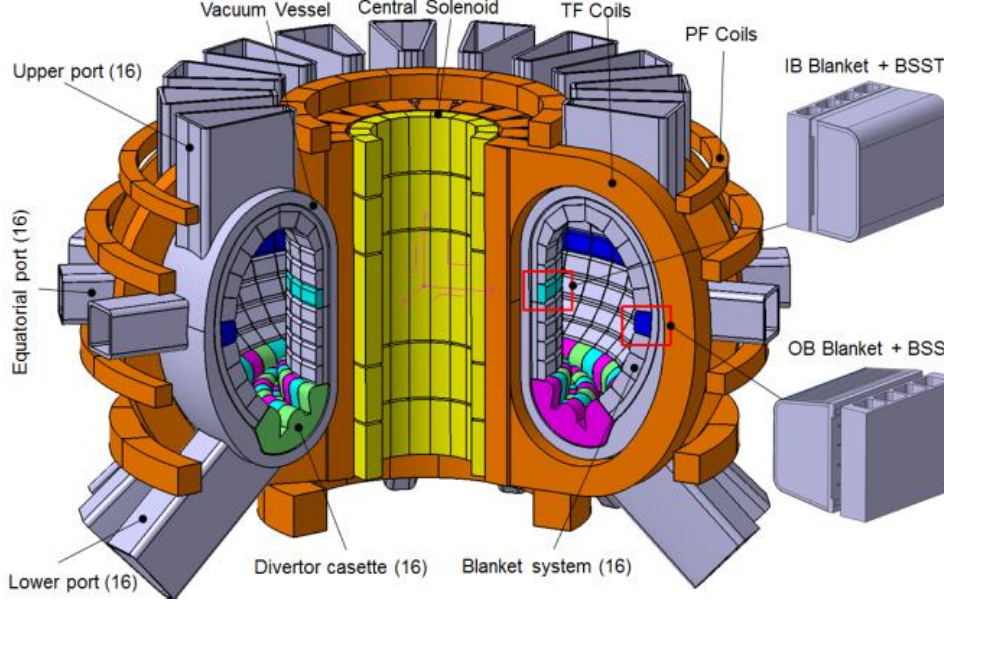
\includegraphics[width=\singleimagewidth]{figures/demo} 
	\caption{An example design of a DEMO reactor with solid breeder blankets shown as inboard (IB) and outboard (OB) blanket components.}
	\label{fig:demo}
\end{figure}

\begin{figure}[ht]
	\centering
	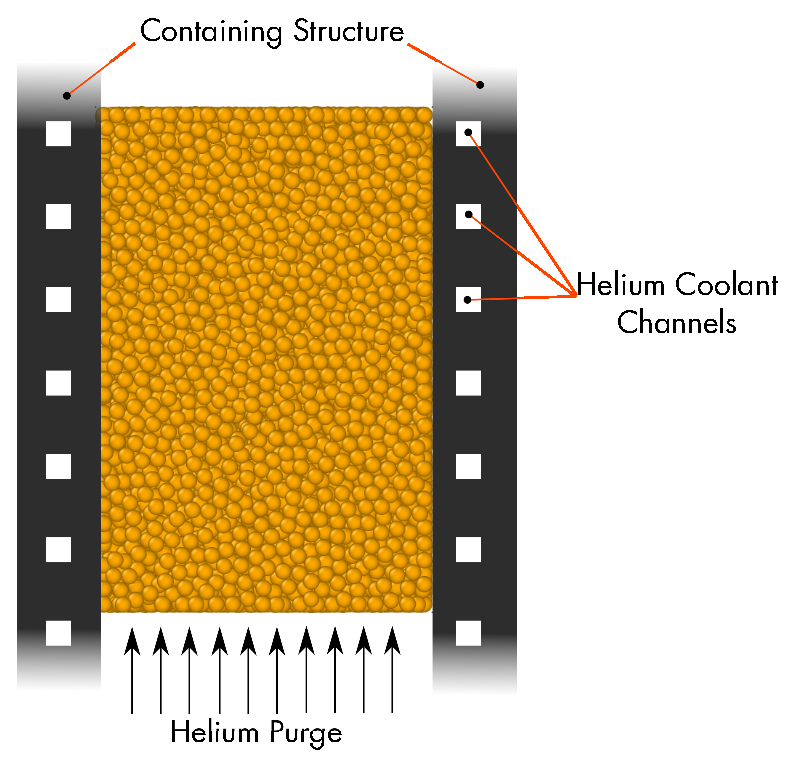
\includegraphics[width=\singleimagewidth]{figures/solid_breeder_sketch} 
	\caption{Sketch of a typical unit of a pebble bed tritium breeding zone. The pebble bed is cooled with contact to the containing structure.}
	\label{fig:solid-breeder-sketch}
\end{figure}

The breeder blanket is a critical piece of engineering technology upon which the success of a fusion power plant largely rests. The successful operation of a breeder will see the device capture the neutrons ejected from the fusion reaction to generate fuel for self-sufficiency via the transmutation of lithium into tritium, act as shield to other sensitive equipment and personnel, and convert energy into extractable heat for electricity production. Figure~\ref{fig:demo} shows an example sketch of a demonstration (DEMO) fusion reactor and the relative location of the breeder blanket modules as they will face the plasma in the torus of the tokamak. The pebble bed (or simply `solid') breeder is one proposed design. Other design concepts see lithium, in liquid form, flowing through the breeder module and then into the fuel processing cycle. These so-called liquid breeders are an entire field of research in their own right and are not discussed in this work.

From the inception of the solid breeder concept, designs have evolved significantly in response to requirements of operation in the harsh fusion environment. Currently, the reference solid breeder design incorporates packed beds of ceramic pebbles (spherical particles) that are filled into containment structures of volumes optimized for thermophysical and tritium responses. The material form of packed beds of spheres has ultimately become the form of choice for solid breeder designers. It is worth noting, however, that other material forms such as sintered pellets or ceramic `foams' have many other advantageous features and should not be completely disregarded. Regardless, many requirements of a solid breeder `material' (the volume of a pebble bed is often considered as a single fictitious material) are satisfied by the ceramic pebble bed. For example, the breeding pebbles can be more easily assembled into complex geometries, the small pebbles provide a sufficient surface-area to volume ratio; have good and customizable (via polydispersity) open-porosity to allow the helium purge gas to wind through and pick up any generated tritium from the solid; and the small size of the pebbles prevent any large thermal gradients from emerging across any single solid material object -- thus increasing the mechanical survivability of the ceramic.

\Cref{fig:solid-breeder-sketch} shows a generic solid breeder volume that is common in all current designs for use in ITER. In a typical design, the breeding zone is subdivided into several regions by cooling plates which contain the pebble bed. Coolant plates are metallic structure which serve as both mechanical and thermal boundaries for the pebble ensemble. In the structure are channels to allow the flow of coolant, typically high-pressure helium. Heat from the pebble bed is conducted into the structure and ultimately into the coolant for the production of electricity. Because the disparity between thermal expansion of the pebble bed and the containing structure, a temperature-dependent mechanical stress acts upon the pebble bed during operation. The stresses lead to rearrangement of packing and may induce crushing of individual pebbles. Flowing through the pebble bed itself is a low-pressure, low-velocity helium purge gas. The purge gas is not intended to act as a heat transfer agent but nevertheless has a large impact on transport of thermal energy between the pebbles and the structure material.

As structural forms of solid breeders converge, we are now able describe the specific details of heat transport and the unique requirements of operating in a fusion reactor which has become a rich field of research.

\subsection{Solid Breeder Thermal Management and Imposed Temperature Window}
High energy (14 MeV) neutrons are ejected from the deuterium-tritium reaction, as described by \Cref{eq:dt-reaction}
\begin{align}
    \mathrm{D} + \mathrm{T}&\xrightarrow{}\ ^4\mathrm{He}+\mathrm{n}+17.58\ \text{MeV} \label{eq:dt-reaction}
\end{align}
thus the breeding blanket will experience high volumetric heating (resulting from secondary $\gamma$ rays and the kinetic energy of neutrons that are carrying away approximately 80\% of the fusion reaction). Pebbles in the breeding blanket transport the deposited heat via inter-particle contact conduction, inter-particle radiation, and convection with the helium purge gas. At the interface with the structural material, similar modes of heat transfer are present: particle-wall contact conduction, particle-wall radiation, and communication via convective helium purge gas. Contact conduction is known to be strongly affected by the packing of the pebble bed (generally described by the packing fraction), and mechanical pressures between pebble bed and structure. The mechanical pressures and packing are expected to evolve during operation of the solid breeder due to phenomena described earlier such as packing rearrangement from large pressures, packing disruption from fragmented pebbles, and pebble sintering. Consequently pebble bed temperatures, linked to the packing, will evolve in ways that are currently not predictable. The major need for temperature prediction is due to its intimate link with tritium release in the ceramic pebbles.

\begin{figure}[ht]
    \centering
    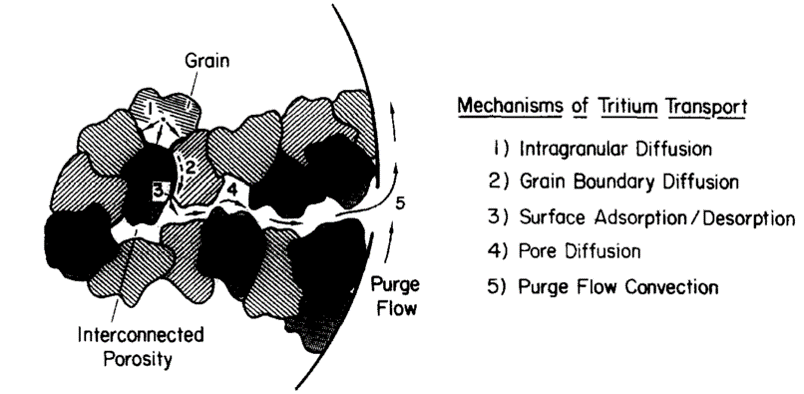
\includegraphics[width=\singleimagewidth]{figures/mechanisms_tritium_transport} 
    \caption{Mechanisms of tritium transport in a single pebble\cite{Federici1990}.}
    \label{fig:mechanisms_tritium_transport}
\end{figure}

To understand the dependence of temperature for tritium release, we can follow the path of a single tritium atom generated in the breeder. Tritium's journey is shown schematically in \Cref{fig:mechanisms_tritium_transport}. As the neutrons bombard the lithiated ceramic, tritium transmuting from lithium is produced internally in pebbles. Tritium then will diffuse slowly through the bulk until reaching a grain boundary. Tritium then moves relatively quickly along the grain boundary until reaching a surface of open porosity where it may desorb into the passing purge gas.\cite{Federici1990} The low-pressure, low-speed purge gas is pumped through the pebble bed to extract the tritium generated and transport it out of the blanket for processing.

Experiments on tritium inventory have attempted to quantify the speeds of tritium release and found that bulk diffusion of tritium, typically the slowest transport mode, is a direct function of temperature.\cite{Franza2013} Thus the lower temperature limit, $T_\text{min}$, of temperature windows for solid breeders, is based on the unacceptable tritium inventory due to slow bulk diffusion. The value of $T_\text{min}$ is generally around \SI{300}{\celsius}.

Using the same model of tritium transport, bulk diffusion also limits the maximum temperature in the solid breeder temperature window. Exposure to prolonged high temperature environments causes individual grains in a pebble to grow. Grain growth therefore extends the characteristic length of the slowest mode of tritium transport. Thus the maximum temperature, $T_\text{max}$, of the operational window for ceramic pebble beds is generally placed around 80\% of the melt temperature of the ceramic, $T_\text{max} = 0.8 T_\text{melt}$, to avoid surface sintering. For many lithium ceramics, this value falls around \SI{950}{\celsius}.

\subsection{Considerations for Temperature Prediction in Solid Breeders}
From the description of the solid breeder structure, we see how the packing structure may change in time due to thermally-induced stresses on the pebble bed. Many experiments have been performed which individually tested the stress-strain response of pebble beds under elevated temperatures. The experiments demonstrated so-called `plastic rearrangement' of the pebble beds wherein rearrangement of the packing structure due to high stress is not recoverable and the amount of plastic strain is dependent on the temperature and the history of stress on the bed. However, in a fusion solid breeder pebble bed, temperatures and stresses are coupled so the single-effect experiments that have been performed are inadequate to predict temperature effects of packing structure rearrangement. Moreover, the relatively narrow temperature window imposed on solid breeders demands high confidence in predictions of temperature distributions in the volume.


\section{Objectives of this Study}\label{sec:intro-scope-of-work}
The goal of this work is to develop a more comprehensive model to predict temperature distributions in packed ceramic pebble beds that accounts for many important phenomena. The model developed will bridge current limitations in pebble bed research, including numerical models of the ceramic pebble bed interactions with and packed bed resettling. Finally, using the models will allow determination of temperature distributions in representative breeder volumes from ITER tritium breeding modules (TBM) and analyze temperature and configuration-dependence on ITER Party designs when resettling occurs.

The path toward satisfying the objective of this work includes several major efforts. These are:
\begin{enumerate}
\item {
    Experimental campaigns and numerical development to increase the accuracy of pebble-scale models. Experimental efforts will both help determine the material properties used in the numerical models as well as allow derivation of a criteria for pebble crushing in an ensemble. Numerically, I will develop and employ models of solid-solid interactions (encompassing pebble-wall and pebble-pebble), solid-fluid interactions, pebble crushing based upon the mechanical interactions, and model fragmentation and discover its impact upon temperature distributions.
}
\item {
    The pebble-scale model will be coupled to fluid flow with efficient bed-scale models of thermo-fluid flow. Two approaches will be concurrently implemented. The steps toward achieving these models includes: adapting and employing two numerical schemes to study packed bed energy transfer with interstitial gas and studying the lumped-capacitance assumption (innate to the particle-scale modeling approach) in a packed bed with high Biot number with nuclear heating.
}
\end{enumerate}
% On the path of pebble-scale modeling development for the solid interacting bodies in the ensemble, I will:
% \begin{enumerate}
% 	\item validate the Hertzian assumption for ceramic pebble interactions with single experiments on crushing pebbles,
% 	\item derive a criteria for pebble crushing in our numeric ensemble based on single pebble experiments,
% 	\item assess the impact of fragment size on packing resettling and its role in thermal transport,
% 	\item calculate the evolving force network and its influence on the heat transport in the pebble bed.
% \end{enumerate}

%After implementing a sophisticated pebble-scale modeling tool, I will show the limitations of the micro-mechanical model when it comes to simulating the heat transfer of a ceramic pebble bed with a creeping helium purge gas. Thus 

% Once the modeling development is complete, the computational tools will be implemented to:
% \begin{enumerate}
% 	\item analyze the reduction in $\keff$ due to broken pebbles,
% 	\item address the overall impact of the helium purge gas on the thermal transport in a bed with evolving morphology,
% 	\item judge the consequences of pebble damage on two ITER-relevant configurations of breeder volumes.
% \end{enumerate}

In summary, understanding the evolution of pebble bed packing structure and its impact on thermophysical properties is critical for solid breeder designers. A more thorough understanding of temperature distributions allows for higher confidence in tritium release from pebble beds as well as the potential for increased power density during operation of the solid breeders. Successful satisfaction of the objectives of this work will see applicable as guidance to solid breeder designers.

One last note: there are other long-term effects expected in the materials experiencing prolonged exposure to cycling irradiation, heat, and stress that have not been discussed here. These loads can lead to thermal ratcheting, irradiation swelling, sintering, or thermally-induced creep which also lead to evolutions in thermophysical properties -- even in the absence of cracked pebbles. These phenomena need to be addressed in time but are, however, beyond the scope of this dissertation. 
